\documentclass[prb,showpacs,floatfix,altaffilletter,amsmath,amssymb,reprint,citeautoscript]{revtex4-1}
\usepackage{custom}
\usepackage{chng}
\usepackage{tikz}
\usetikzlibrary{optics}


\begin{document}

\title{Amplificatore lock-in ad allineamento in fase per la misura dei coefficienti di Fresnel su cristalli non dielettrici}
\author{Mattia Sotgia}
\email{s4942225@studenti.unige.it}
\author{Francesco Polleri}
\email{s5025011@studenti.unige.it}
\affiliation{Università degli Studi di Genova, Dipartimento di Fisica}
\date{\today}

\begin{abstract}
    Presentiamo la progettazione e la realizzazione di un esperimento per la misura dei coefficienti di Fresnel di un film sottile di cristallo di Silicio (c-Si) e su un sottile campione di oro (Au). La misura è effettuata sfruttando un sistema di accoppiamento di fase lock-in\cite{scofieldFrequencydomainDescriptionLockin1994} che permette una migliore reiezione in frequenza del rumore. Descriviamo la progettazione del sistema di misura, e infine una descrizione e discussione dei risultati, confrontando con modelli teorici. Il sistema descritto permette di effettuare misure con sufficiente precisione dei coefficienti di Fresnel $R_s$ e $R_p$, permettendo di ottenere i coefficienti di riflessione e trasporto $n_\text{c-Si}/k_\text{c-Si}$ e $n_\text{Au}/n_\text{Au}$. Per il cristallo di silicio (c-Si) possiamo anche inferire il valore dello spessore del film di ossido di silicio ($\mathrm{SiO_2}$) depositato sul substrato di silicio.
    % \comment{Aggiungere anche alcuni commenti riguardo ai risultati ottenuti}
\end{abstract}
\maketitle

\section{Introduzione} 

L'utilizzo di un sistema sensibile allo sfasamento, come un amplificatore lock-in, può risultare molto comodo in applicazioni di misura in cui si fa utilizzo di segnali luminosi, in particolar modo se questi segnali sono periodici. In questo modo è infatti possibile ridurre sufficientemente i disturbi e le interferenze prodotte dal rumore esterno, che in un ambiente di laboratorio possono essere molteplici, e inoltre permette anche di controllare e ridurre fonti di rumore che sono invece causate dal sistema stesso, che sono di carattere aleatorio. Poiché il processo di lock-in consiste matematicamente nello spostare in frequenza un segnale, questo allora può anche essere utilizzato anche con segnali che sono teoricamente in continua, modulandoli con un segnale a frequenza definita o nota, in modo da spostarli nello spettro in una regione a minore rumore, e poi riportandolo alla frequenza di partenza, rimodulando il segnale fisico con un riferimento in fase. Considerando allora un sistema che permette di generare e di acquisire con una frequenza definita, possiamo infatti ridurre molti di questi contributi di rumore, e quindi incrementare il rapporto tra segnale e rumore (SNR). 

Nel caso specifico della misura che vogliamo compiere il segnale è effettivamente un segnale in continua, dato da una sorgente coerente di luce sufficientemente collimata. Questa è polarizzata e quindi fatta incidere sul campione cristallino. Il segnale quindi riflesso è quindi acquisito. Questo sistema è però estremamente soggetto a rumore, caratteristico dei segnali a bassissima frequenza. La soluzione allora è individuabile nel spostare il segnale di riferimento da $\nu=\SI{0}{\Hz}$ a frequenza che siano in una regione dello spettro a basso rumore. Quindi convertire poi il segnale in continua sfruttando l'accoppiamento in fase con un riferimento e infine riportare il segnale alla stessa frequenza di partenza. 

Questo sistema così progettato può essere allora utilizzato per effettuare misure dei coefficienti di Fresnel\cite{fresnelCalculationTintsThat2021,fresnelNoteCalculTeintes1821} $r$ e $R$ dati differenti campioni di cristalli, conduttori elettrici. Si sfrutta il sistema descritto in quanto il segnale del laser, se studiato in continua, può presentare distorsioni legate al comportamento sub-ottimale a basse frequenze, dove la maggior parte delle fonti di rumore sono presenti, e invece spostare il segnale in frequenza in una regione dello spettro con un migliore SNR. L'obiettivo scientifico è quindi quello di poter caratterizzare le curve di Fresnel per i coefficienti di riflessione per due campioni. 

Il documento è diviso in una parte immediatamente successiva che descrive a grandi linee alcune formalizzazioni del sistema utilizzato, a cui segue poi un dettaglio sulla teoria fisica del fenomeno studiato, per definire al meglio le osservabili in questione, e infine una descrizione e caratterizzazione dell'esperimento, e una breve discussione sulle modalità di analisi dati e sui risultati ottenuti. 

\paragraph*{Teoria del lock-in} 
Il segnale fisico (nel caso specifico il segnale è dato dal fascio luminoso) è modulato su un'onda sinusoidale\footnote{Nel caso sperimentale il segnale è modulato su un'onda quadra, essendo utilizzato un \emph{chopper}, ma la matematica si complicherebbe, riportiamo quindi eventuali correzioni alla teoria generale nelle note.} come $V_0 \cos(\omega_\mathrm{r} t)$, dove il pedice r indica che si tratta anche della frequenza con cui andiamo poi a stimolare il riferimento che forniamo al \emph{lock-in}. $V_0$ è l'ampiezza del segnale fornita al sistema. 

Il sistema complessivo avrà allora un output della forma $V_\mathrm{out} \cos(\omega_\mathrm{r} t + \phi_\mathrm{out}),$ dove una fase arbitraria, ma non casuale, può essere in generale aggiunta dal processo fisico che stiamo studiando. Il segnale di riferimento fornito in ingresso al lock-in allora deve anche esso presentare una fase $\phi_\mathrm{ref}$ per fare in modo che sia accoppiato al segnale che viene letto dal rivelatore. 

Il segnale fisico che allora avremo in ingresso al lock-in è dato da un primo stadio di amplificazione, che compie l'operazione \begin{equation}
    V_\mathrm{out} \cos(\omega_\mathrm{r} t + \phi) \to s_\mathrm{in}(t) = G_\mathrm{amp}V_\mathrm{out} \cos(\omega_\mathrm{r} t + \phi),
\end{equation} dova anche un eventuale rumore $n(t)$ viene portato in $G_\mathrm{amp}n(t)$. Successivamente all'accoppiamento in fase avremo il prodotto tra $s_\mathrm{in}(t)r(t)$, con $r(t)$ il riferimento fornito dopo lo stadio di amplificazione. Come riportato in ref. \onlinecite{scofieldFrequencydomainDescriptionLockin1994}, dopo un ultimo stadio passa-basso ottenuto con un filtro LPF (\emph{Low Pass Filter}), il sistema avrà ridotto notevolmente le componenti di rumore casuali, ma resterà ancora caratterizzato dalle componenti sistematiche del rumore \begin{equation}
    s_\mathrm{LPF}(t) = \frac{G V_\mathrm{out}}{2} \cos(\phi) + \frac{G \eta(\omega_0)}{2}\cos(\phi_\mathrm{n}(\omega_0)), \label{eq:s_LPF}
\end{equation} dove indichiamo con $\eta(\omega_0)$ la componente di rumore che corrisponde alla frequenza a cui sta operando il sistema lock-in, che non può essere eliminata automaticamente, ma può essere ridotta scegliendo una precisa regione nel dominio delle frequenze dove sappiamo che abbiamo meno rumore (evitiamo ad esempio di scegliere come frequenza di modulazione la $\SI{50}{\Hz}$).

Per questa breve introduzione abbiamo trascurato di trattare un segnale di riferimento che non è sinusoidale ma può essere ad esempio un'onda quadra. Questa spettralmente presenta non solo un picco principale, ma introduce anche armoniche successive a quella principale $\omega_0$, che implicano la necessità di una migliore calibrazione del sistema. Per questo la frequenza di operazione del lock-in $\omega_0$ dovrà essere calibrata assieme alla frequenza di taglio del LPF per tagliare con maggiore efficienza le armoniche a frequenze più alte.  

Un altro termine su cui abbiamo controllo è infine la differenza di fase $\phi_\mathrm{out} - \phi_\mathrm{ref} = \phi$ della \eqref{eq:s_LPF}, dove osserviamo inoltre che massima efficienza per il sistema si ottiene per $\phi\ll 1$, per cui $\cos\phi\simeq1$.

\section{Teoria}

Prima di presentare la progettazione e caratterizzazione del sistema procediamo a definire con un po' più di rigore la misura che vogliamo effettuare e la teoria sottostante. 

Considerato un fascio di luce generico ogni possibile angolo di polarizzazione è espresso dalla combinazione lineare di due vettori di una base di polarizzazione, che possono essere scelti in modo da essere ortonormali, posto uno parallelo, denotato da $p$, e l'altro ortogonale al piano di incidenza, denotato da $s$. Queste due polarizzazioni prendono anche altre definizioni, per esempio descrivendo quale campo è ortogonale al piano di incidenza. Avremo allora che onde polarizzate $p$ sono anche definite \emph{transverse-magnetic} (TM), e onde polarizzate $s$ sono definite \emph{transverse-electric} (TE). La percentuale di luce riflessa, dato un campione di materiale X, è dipendente dal grado di polarizzazione ed espressa dalle relazioni ottenute da Fresnel\cite{fresnelCalculationTintsThat2021,fresnelNoteCalculTeintes1821}, per cui avremo che il coefficiente di riflessione per onde TE è dato come \begin{equation}
    r_\mathrm{s} = \frac{\underline{n}_1\cos\theta_i - \underline{n}_2\cos\theta_t}{\underline{n}_1\cos\theta_i + \underline{n}_2\cos\theta_t},
    \label{eq:fresnel_rs}
\end{equation} mentre per le onde TM è dato come \paragraph*{}\begin{equation}
    r_\mathrm{p} = \frac{\underline{n}_2\cos\theta_i - \underline{n}_1\cos\theta_t}{\underline{n}_2\cos\theta_i + \underline{n}_1\cos\theta_t}. 
    \label{eq:fresnel_rp}
\end{equation} In generale il coefficiente $n_i$ indica il coefficiente di rifrazione del materiale che si sta considerando. Tale coefficiente è generalmente reale, ma per materiali conduttori, si è osservata la necessità di estendere la teoria\cite{attwoodSoftXRaysExtreme1999} introducendo il coefficiente complesso $\underline n = n + ik$, dove $k$ è una quantità caratteristica del materiale in considerazione, come anche $n$, determinabili sperimentalmente. Generalizziamo allora le \eqref{eq:fresnel_rs} e \eqref{eq:fresnel_rp} considerando indici complessi. Questi sono allora effettivamente funzioni a variabile complessa. La frazione riflessa, detta riflettanza, è data allora da \begin{equation}
    R_i= \qty|r_i|^2, \quad i = \mathrm{s,p}
\end{equation} e tende a 1 per l'angolo di riflessione che tende a \SI{90}{\degree}.

Nelle relazioni \eqref{eq:fresnel_rs} e \eqref{eq:fresnel_rp} in realtà è possibile avere funzioni ad una sola variabile (che può essere sia $\theta_i$ che $\theta_t$, generalmente con la scelta di poter controllare l'angolo di incidenza del fascio luminoso si considera $\theta_i$) ricordando che dalle leggi di Snell \begin{equation}
    \cos\theta_t = \sqrt{1-\qty(\frac{\underline n_1}{\underline n_2}\sin\theta_i)^2}.
    \label{eq:snell}
\end{equation}

Questo modello è sufficientemente valido per quando l'interfaccia che si sta studiando è semplice, e il materiale su cui il fascio di luce è fatto incidere sufficientemente profondo da disperdere al suo interno la maggior parte della radiazione incidente, e non avere quindi altri fenomeni di riflessioni secondarie. Questo è quindi valido per il caso del campione di oro (fig. \ref{fig:Au}).

Ci possono essere però alcune situazioni in cui il modello semplificato non è sufficiente, sopratutto quando il materiale in questione, per quanto preparato con estrema precisione, presenta sottili strati superficiali di materiale con indice di rifrazione differente. Questo è vero in particolar modo per il cristallo di silicio, c-Si, per il quale si ha un deposito di ossido di silicio $\mathrm{SiO_2}$ (vedi figura \ref{fig:c-Si}) con uno spessore $d>\SI{1}{\nano\metre}$ sufficiente per avere fenomeni di riflessione multipla nel sottile film interposto ad ambiente (aria, con indice di rifrazione noto, $n_\mathrm{Air}$) e il substrato di c-Si, con indice $\underline n_\text{c-Si}$. La teoria che ne segue si complica. Dobbiamo allora introdurre il modello a tre fasi (\emph{three-phases model}\cite{cobetEllipsometrySurveyConcept2018, hinrichsEllipsometryFunctionalOrganic2018, yehOpticalWavesLayered1988})\footnote{Nel caso della ref. {\onlinecite{yehOpticalWavesLayered1988}} la convensione sul segno dell'esponenziale è differente da quella utilizzata invece dalla ref. {\onlinecite{hinrichsEllipsometryFunctionalOrganic2018}}, ma questo è indifferente considerato che l'esponenziale complesso è periodico $2\pi$. Nella \eqref{eq:three_phase_model} utilizziamo la convenzione presentata nella seconda} per cui i coefficienti introdotti in (\ref{eq:fresnel_rs}-\ref{eq:fresnel_rp}) non sono più sufficienti, ma dobbiamo introdurre i coefficienti \begin{equation}
    r = \frac{r_{al} + r_{ls}e^{2i\beta}}{1 + r_{al}r_{ls}e^{2i\beta}},\label{eq:three_phase_model}
\end{equation} valida sia per i modi TE che per i modi TM di oscillazione. I coefficienti $r_{al}$ e $r_{ls}$ hanno la stessa forma di (\ref{eq:fresnel_rs}-\ref{eq:fresnel_rp}), considerando questa volta che però gli angoli di incidenza sono relativi all'interfaccia che si sta considerando: aria/$\mathrm{SiO_2}$ nel caso di $r_{al}$, e $\mathrm{SiO_2}$/c-Si nel caso di $r_{ls}$. Il coefficiente $\beta$ è invece indicativo della differenza di fase legata al cammino ottico allinterno del layer sottile depositato sulla superficie del cristallo (si veda l'eq. (1.16) di ref. \onlinecite{hinrichsEllipsometryFunctionalOrganic2018}), ed è espresso come \begin{equation}
    \beta = \frac{2\pi}{\lambda} d \sqrt{\underline n_l^2 - \underline n_a^2 \sin^2\phi_a}.
\end{equation} Osserviamo subito che il modello è sicuramente più complesso del precedente, il che comporterà la necessità di fare assunzioni in fase di analisi dati per poter ottenere dei risultati corretti. 

\begin{figure}
    \centering
    \subfloat{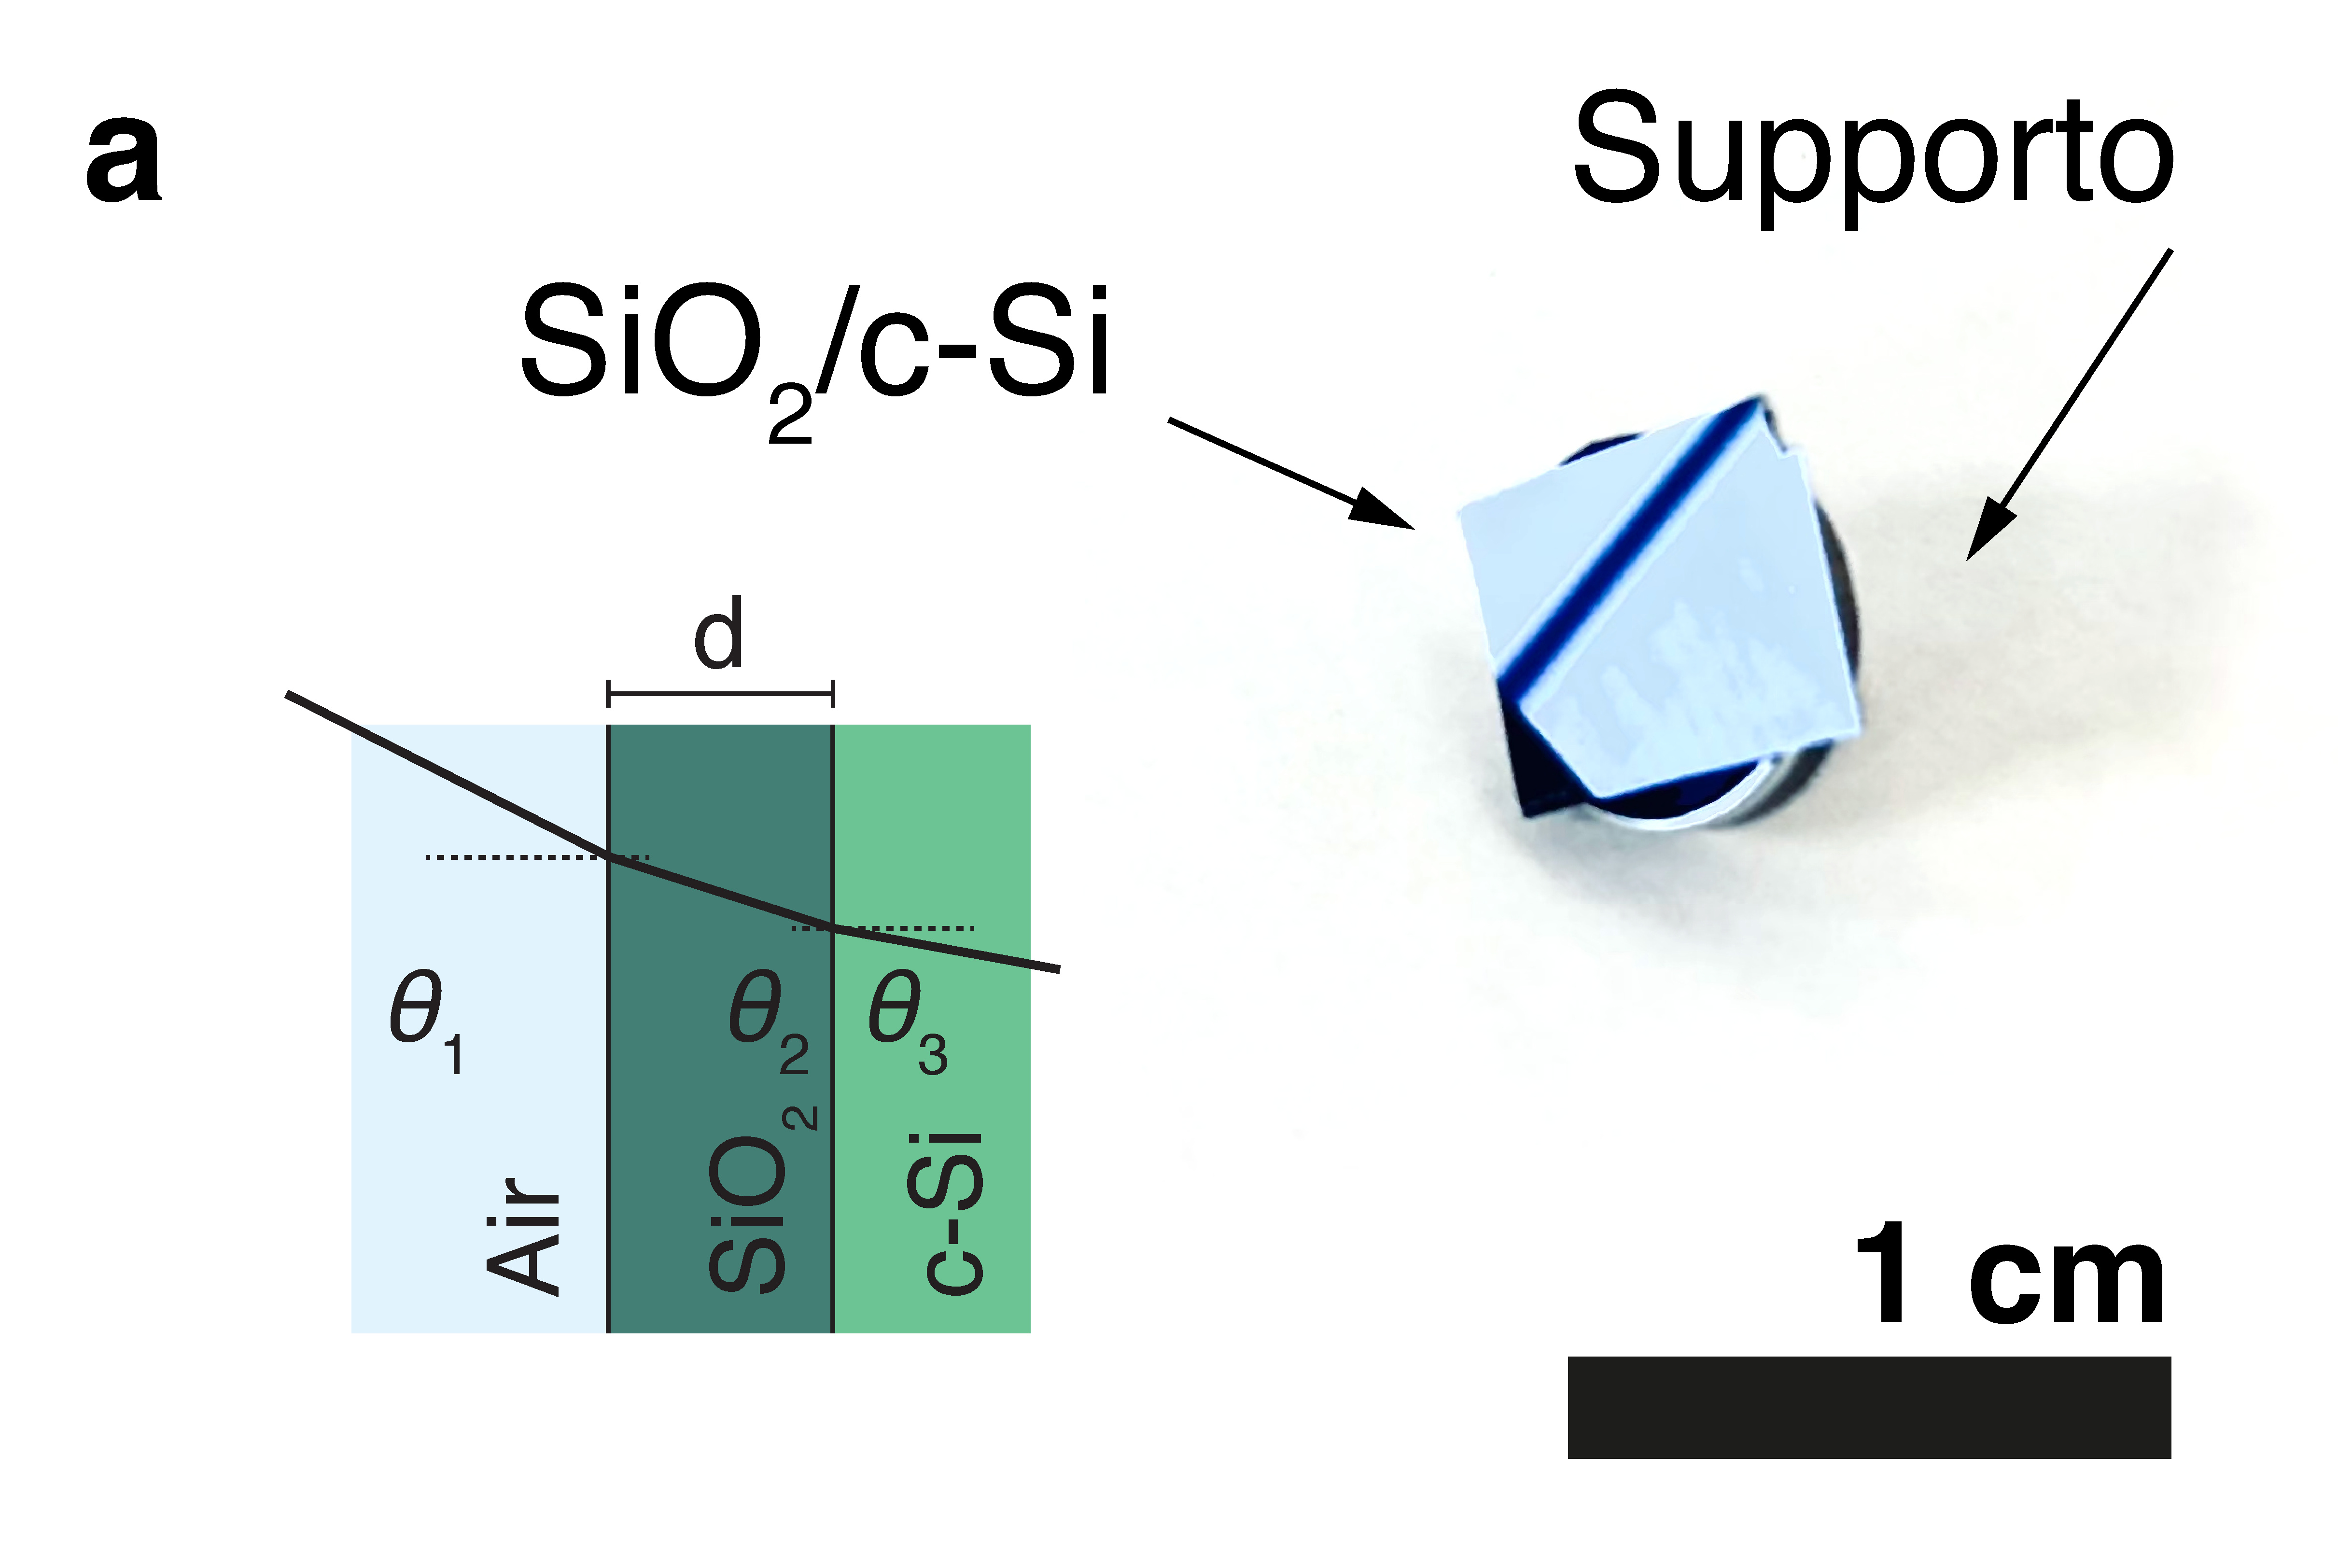
\includegraphics[width=0.9\linewidth,trim={0 4cm 0 0}]{figures/c-Si.pdf}\label{fig:c-Si}}
    
    \subfloat{\includegraphics[width=0.9\linewidth]{figures/Au_sample.pdf}\label{fig:Au}}
    \caption{\ref{sub@fig:c-Si} Campione di  cristallo di Silicio montato sul supporto necessario per poter effettuare le misure. A lato è anche schematizzata la struttura a layer dell'interfaccia del c-Si con l'aria, a cui è interposto un sottile strato di $\mathrm{SiO_2}$ che cambia quindi l'angolo con cui la luce incide sul silicio. \ref{sub@fig:Au} Campione di oro e schema della struttura dell'interfaccia aria/oro. Il campione è montato al centro del goniometro. Sullo stesso supporto è possibile anche fissare il campione di c-Si.}
    \label{fig:c-Si/Au_samples}
\end{figure}

\section{L'esperimento}

L'esperimento è costituito da un goniometro da banco ottico con precisione di \ang{0;20} su entrambi gli angoli (incidenza e riflessione) rispetto al campione posizionato al centro. Il goniometro è assicurato ad un banco ottico sfruttato come supporto per l'intero setup, controllato localmente da un computer con LabView, che permette anche l'acquisizione dei dati. Uno dei due bracci del goniometro ospita il supporto per la sorgente laser, mentre l'altro ospita il fotodiodo rivelatore. Sul cammino ottico del fascio di luce è inoltre inserito un modulatore in frequenza, immediatamente vicino alla sorgente, e due filtri polarizzatori, posizionati dopo il \emph{chopper} ma prima del campione al centro del sistema. Quello più lontano dalla sorgente è l'ultima lente che il fascio attraversa prima di incidere sul campione, e definisce quindi il piano di polarizzazione dell'onda incidente. Quello immediatamente precedente è invece necessario per ridurre l'intensità della luce incidente sul campione e della frazione di luce che poi colpisce il fotodiodo per evitare una eccessiva usura del campione e dello strumento di misura, ed inoltre per non avere un segnale eccessivamente grande in ingresso sul sistema. La scheda di acquisizione è infatti limitata in ampiezza a circa \SI{10}{\volt}, per cui la scelta dell'angolo relativo tra le due lenti polarizzatrici è importante per poter controllare l'intensità secondo queste limitazioni sperimentali. Uno schema del setup utilizzato è in figura \ref{fig:setup}, mentre in figura \ref{fig:setup_on} troviamo una fotografia del setup in utilizzo. 

\paragraph{Sorgente} La sorgente è costituita da un laser verde estremamente collimato \comment{Inserire qua eventuali caratteristiche precise}, alimentato in corrente continua 


\begin{figure*}
    \centering
    \subfloat{\includegraphics[height=5cm,page=1]{figures/setup.pdf}\label{fig:setup}}
    \subfloat{\includegraphics[height=5cm,page=2]{figures/setup.pdf}\label{fig:setup_on}}
    \caption{\ref{sub@fig:setup} Schema del setup utilizzato. $P_1$ è il primo polarizzatore, che controlla l'intensità del fascio, insiema a $P_2$, che inoltre permette di definire la polarizzazione della luce, ricordando che l'intensità dopo due filtri è proporzionale al $\cos\theta_{1,2}$ dell'angolo compreso tra i due filtri. \ref{sub@fig:setup_on} Fotografia del setup utilizzato durante una misura. }
    \label{fig:setup_and_photo}
\end{figure*}








\begin{figure}
    \centering
    \includegraphics[width=\linewidth,trim={0 8cm 0 0}]{figures/photoDiode.pdf}
    \caption{Immagine del fotodiodo utilizzato per la acquisizione dei dati. Il laser colpisce ortogonalmente il cristallo semiconduttore , che ha una apertura angolare di circa \SI{2}{\degree}, sulla quale la risposta è pressoché uniforme, come possiamo dedurre anche dal grafico, ad eccezione fatta per le regioni ai bordi, evidenziate in verde, per le quali interviene il fattore di forma del fascio di luce laser, che per quanto estremamente collimato presenta una distribuzione approssimativamente gaussiana, della quale stiamo osservando le code.}
    \label{fig:photo-diode}
\end{figure}







%%%%%% TODO
\iffalse

\paragraph*{L'esperimento} 
L'esperimento è definito da una sorgente di luce coerente debolmente polarizzata, trasmessa e incidente \replace[FP]{sul bersaglio semitrasparente, e il segnale riflesso è in linea con il rivelatore che permette di misurare l'intensità del fascio incidente.È possibile interporre sul cammino ottico del fascio laser un rivelatore di intensità luminosa, ovvero un fototransistor, e delle lenti polarizzatrici.}{su un bersaglio semitrasparente che genera un fascio riflesso che è in linea con un rivelatore di intensità luminosa costituito da un fototransistor. Sul cammino ottico di questo fascio è inoltre possibile inserire delle lenti polarizzatrici.}

Il segnale luminoso è prodotto da una sorgente coerente \comment[MS]{Dobbiamo descrivere accuratamente le caratteristiche del laser utilizzato.} verde, controllato da un segnale periodico che ne permette l'accoppiamento in fase con il ricevitore.\comment[FP]{Parliamo qui del chopper o dopo?} In questo modo possiamo ridurre gli effetti aleatori legati alla produzione e alla ricezione del segnale fisico. Il segnale luminoso è quindi fatto passare in aria e attraverso \replace[FP]{un primo filtro polarizzatore: l'inserimento di questa componente ottica permette di controllare l'angolo con cui la radiazione incidente è polarizzato.}{due filtri polarizzatori. } Infatti il laser produce un segnale coerente che dovrebbe essere idealmente non polarizzato, ma che realmente \replace[FP]{è invece polarizzato.}{invece lo è almeno in parte} 





\begin{figure*}
    \centering
    \subfloat[]{\includegraphics[width=0.45\linewidth]{figures/phase_ratio_Air.Au.pdf}\label{fig:Air.Au.rp/rs}}
    \subfloat[]{\includegraphics[width=0.45\linewidth]{figures/phase_ratio_Air.SiO2.Si.pdf}\label{fig:Air.SiO2.Si.rp/rs}}
    \caption{\ref{sub@fig:Air.Au.rp/rs}\ref{sub@fig:Air.SiO2.Si.rp/rs}\comment[MS]{Need clear explanation (is actually useful data)}}
    \label{fig:enter-label}
\end{figure*}

\appendix

\fi

\bibliography{references/brewster_research}

\end{document}
